\documentclass[9pt,twocolumn,a4paper,landscape]{extarticle}
%
\usepackage[dvipdfmx]{graphicx}
\usepackage{latexsym}
\usepackage{amsmath,amssymb}
\usepackage[cmbtt]{bold-extra}
\usepackage{bm}
\usepackage{graphicx}
\usepackage{ascmac}
\usepackage{indentfirst}
%
\setlength{\columnsep}{3zw}
\setlength{\topmargin}{20mm}
\addtolength{\textheight}{-40mm}
\addtolength{\topmargin}{-1.55in}
\setlength{\headsep}{10pt}
\setlength{\textheight}{190mm}
\setlength{\oddsidemargin}{-15mm}
\setlength{\textwidth}{279mm}
%
\newcommand{\divergence}{\mathrm{div}\,}
\newcommand{\grad}{\mathrm{grad}\,}
\newcommand{\rot}{\mathrm{rot}\,}
%
\setcounter{tocdepth}{3}
\usepackage[dvipdfmx,
bookmarks=true,
anchorcolor=blue,
linkcolor=blue,
urlcolor=blue,
colorlinks=true,
bookmarksopen=true,
]{hyperref}


% Listingsの設定
\usepackage{ascmac,here,txfonts,txfonts}
\usepackage{listings,jlisting}
\usepackage[dvips]{color}
\lstset{
  breaklines = true,
  language=c++,
  captionpos=b,
  basicstyle={\ttfamily \footnotesize},
  commentstyle={\itshape \color[cmyk]{1,0.4,1,0}},
  keywordstyle={\ttfamily \color[cmyk]{0.3,0.9,0,0}},
  stringstyle={\ttfamily \color[rgb]{0.8,0,0}},
  frame=tlrb,
  framesep=5pt,
  showstringspaces=false,
  numbers=left,
  stepnumber=1,
  numberstyle=\tiny,
  tabsize=2,
  xleftmargin=5mm,
}
\usepackage{fancyhdr}
\pagestyle{fancy}
\lhead{\empty}
\chead{FCCPC\_arroy (Tokyo Institute of Technology)}
\rhead{\thepage}
%\lfoot{FCCPC Library}
\lfoot{\empty}
\cfoot{\empty}
\rfoot{\empty}
%\rfoot{\thepage}
\renewcommand{\footrulewidth}{0.0pt}
\renewcommand{\headrulewidth}{0.1pt}
%\footskip 24pt
%
\begin{document}
\tableofcontents
\newpage
\section{準備}
\subsection{Caps LockをControlに変更}
2つ
\begin{enumerate}
  \item
    変更
    \begin{lstlisting}
setxkbmap -option ctrl:nocaps;
    \end{lstlisting}
    元に戻す
    \begin{lstlisting}
setxkbmap -option;
    \end{lstlisting}
  \item
    上でダメな場合
    \begin{lstlisting}
xmodmap -e 'remove Lock = Caps_Lock';
xmodmap -e 'add Control = Caps_Lock';
xmodmap -e 'keysym Caps_Lock = Control_L';
    \end{lstlisting}
\end{enumerate}

\subsection{init.el}
linumはemacs24のみ\par
\lstinputlisting[language=Lisp]{others/init.el}

\subsection{tpl.cpp}
\lstinputlisting{others/tpl.cpp}

\subsection{get input}
\begin{lstlisting}
wget -r http://(url of sample input)
\end{lstlisting}

\subsection{alias}
\begin{lstlisting}
alias g++='g++ -g -O2 -std=gnu++0x -Wl,-stack_size,64000000';
alias emacs='emacs -nw';
\end{lstlisting}


\section{文字列}
\subsection{マッチング}
\subsubsection{複数文字列マッチング(Aho-Corasick法)}
$O(N+M)$\par
\lstinputlisting{string/aho_corasick.cpp}

\subsection{Suffix Array}
find\_string() : $O(|T|\log |S|)$\par
S中にTが含まれないなら-1, 含まれるならその先頭.\par
LCS() : $O(|S+T|)$\par
最長共通部分文字列. (先頭, 長さ)を返す.

\lstinputlisting{string/sa.cpp}

\subsection{回文長(Manacher)}
$O(N)$\par
各文字を中心とした時の回文の最長の半径.\par
偶数長の回文はダミーを挟むことで求められている.\par
\lstinputlisting{string/manacher.cpp}


\section{グラフ}
\lstinputlisting{graph/graph.cpp}
\subsection{強連結成分分解}
\subsubsection{関節点}
$O(E)$\par
ある関節点uがグラフをk個に分割するときartにはk-1個のuが含まれる. 不要な場合はuniqueを忘れないこと.\par
\lstinputlisting{graph/articulation.cpp}

\subsubsection{橋}
$O(V+E)$\par
\lstinputlisting{graph/bridge.cpp}

\subsubsection{強連結成分分解}
$O(V+E)$\par
\lstinputlisting{graph/strongly_connected_component.cpp}

\subsubsection{無向中国人郵便配達問題}
$O(om\log n+o^22^o)$, $-O2$で$o\leq 18$程度が限界
\lstinputlisting{graph/chinese_postman.cpp}
\subsubsection{全点対間最短路(Johnson)}
$O(max(VE\log V, V^2))$
\lstinputlisting{graph/johnson.cpp}
\subsubsection{無向グラフの全域最小カット}
$O(V^3)$
\lstinputlisting{graph/minimum_cut.cpp}

\subsection{フロー}
\subsubsection{最大流}
$O(EV^2)$\par
\lstinputlisting{graph/flow/max_flow.cpp}

\subsubsection{二部マッチング}
$O(EV)$\par

\lstinputlisting{graph/flow/bi_matching.cpp}
\subsubsection{最小費用流}
$O(FE\log V)$\par
\lstinputlisting{graph/flow/minimum_cost_flow.cpp}

\subsubsection{Gomory-Hu木}
$O(V MAXFLOW)$
\lstinputlisting{graph/flow/gomory_hu.cpp}

\subsection{木}
\subsubsection{木の直径}
ある点(どこでもよい)から一番遠い点aを求める. 点aから一番遠い点までの距離がその木の直径になる.\par
\subsubsection{最小全域木}
\lstinputlisting{graph/minimum_spanning_tree.cpp}
\subsubsection{最小全域有向木}
$O(VE)$
\lstinputlisting{graph/ms_arborescence.cpp}
\subsubsection{最小シュタイナー木}
$O(4^{|T|}V)$ \par
gは無向グラフの隣接行列. Tは使いたい頂点の集合.\par
\lstinputlisting{graph/minimum_steiner_tree.cpp}
\subsubsection{木の同型性判定}
順序付き$O(n)$\par
順序なし$O(n\log n)$
\lstinputlisting{graph/tree_isomorphism.cpp}

\subsubsection{HL分解}
\lstinputlisting{graph/heavy_light_decomposition.cpp}

\subsubsection{重心分解}
\lstinputlisting{graph/centroid_decomposition.cpp}
\subsection{彩色数}
\subsubsection{包除原理}
$O(2^VV)$\par
N[i] := iと隣接する頂点の集合(iも含む)\par
\lstinputlisting{graph/graph_coloring.cpp}
\subsubsection{極大独立集合}
\lstinputlisting{graph/indsets.cpp}



\section{数学}
\subsection{整数}
\subsubsection{剰余}
\lstinputlisting{math/modulo/number_theory.cpp}

\subsubsection{カタラン数}
$n\leq 16$程度が限度. $n\geq 1$について以下が成り立つ.
\begin{eqnarray*}
  C_n &=& \frac{1}{n+1}\binom{2n}{n}\\
      &=& \binom{2n}{n}-\binom{2n}{n-1}\\
\end{eqnarray*}
nが十分大きいとき, カタラン数は以下に近似できる.
\begin{eqnarray*}
  C_n &=& \frac{4^n}{n^{3/2}\sqrt{\pi}}\\
\end{eqnarray*}
()を正しく並べる方法, 二分木, 格子状の経路の数え上げ, 平面グラフの交差などに使われる.\\
$C_3=5$\\
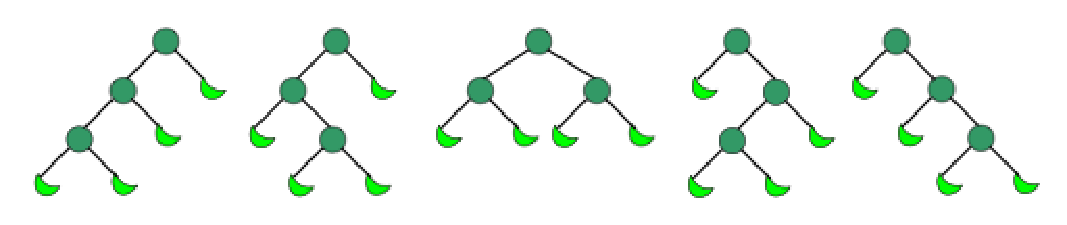
\includegraphics[width=9cm, clip]{images/Catalan_tree.eps}\\
$C_4=14$\\
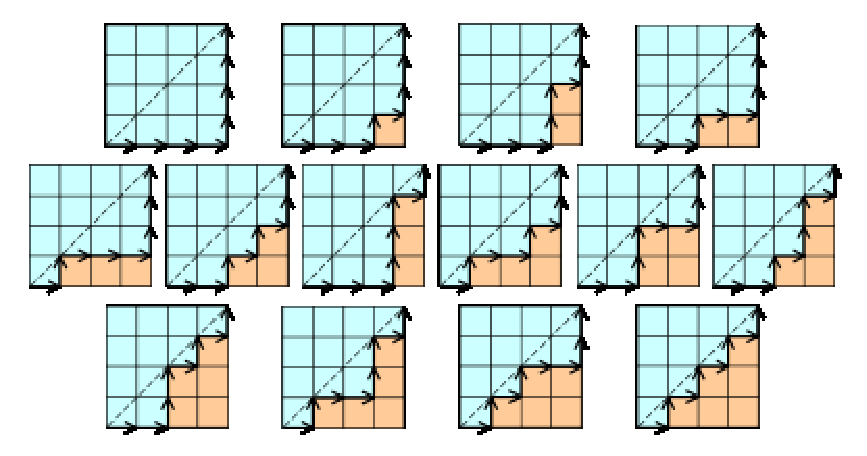
\includegraphics[width=9cm, clip]{images/Catalan_graph.eps}\\

\subsubsection{乱数(xor shift)}
周期は$2^{128}-1$
\lstinputlisting{math/xor_rand.cpp}

\subsubsection{確率的素数判定(Miller-Rabin法)}
$O(k\log^3n)$\par
合成数を素数と判定する確率は最大で$4^{-k}$\\
\lstinputlisting{math/miller_rabin.cpp}

\subsection{多項式}
FFTは基本定数重めなのでTLEに注意する.
\subsubsection{FFT(complex)}
$O(N \log N)$\par
複素数を用いたFFT. 変換するvectorのサイズは2の冪乗にすること.
\lstinputlisting{math/fft.cpp}

\subsubsection{FFT(modulo)}
$O(N \log N)$\par
剰余環を用いたFFT(FMT). 変換するvectorのサイズは2の冪乗にすること. modは$a*2^e+1$の形.\\
\lstinputlisting{math/fmt.cpp}

\subsubsection{積(FMT)}
$O(N \log N)$\par
$poly\_mul()$が必要.
\lstinputlisting{math/poly_mul.cpp}

\subsubsection{逆元(FMT)}
$O(N \log N)$\par
$extgcd()$, $mod\_inverse()$, $poly\_mul()$, $fmt()$が必要.
\lstinputlisting{math/poly_inv.cpp}

\subsubsection{平方根(FMT)}
$O(N log N)$\par
$extgcd()$, $mod\_inverse()$, $poly\_inv()$, $poly\_mul()$, $fmt()$が必要.
\lstinputlisting{math/poly_sqrt.cpp}


\subsection{行列}
\lstinputlisting{math/matrix/matrix.cpp}

\subsubsection{線形方程式の解(Givens消去法)}
$O(N^3)$
\lstinputlisting{math/matrix/givens.cpp}

\section{幾何}
\lstinputlisting{geometry/geometry.cpp}
\subsection{点}
\lstinputlisting{geometry/point.cpp}
\subsection{直線と線分}
\lstinputlisting{geometry/line.cpp}
\subsection{円}
\lstinputlisting{geometry/circle.cpp}
\subsection{多角形}
\lstinputlisting{geometry/polygon.cpp}
\subsubsection{凸包}
\lstinputlisting{geometry/convex_hull.cpp}
\subsubsection{最近点対}
だいたい$O(n\log n)$, 最悪縦1列に並んでる場合$O(n^2)$
\lstinputlisting{geometry/closest_pair.cpp}
\subsubsection{点-多角形包含判定}
$O(n)$
\lstinputlisting{geometry/contains.cpp}
\subsubsection{凸多角形の共通部分}
$O(n+m)$
\lstinputlisting{geometry/convex_intersect.cpp}
\subsubsection{凸多角形の直径}
$O(n)$
\lstinputlisting{geometry/convex_diameter.cpp}
\subsubsection{ドロネー三角形分割(逐次添加法)}
$O(n^2)$
\lstinputlisting{geometry/delaunay.cpp}

\section{データ構造}
\subsection{Union-Find木}
\lstinputlisting{data-structure/union_find_tree.cpp}
\subsection{Binary-Indexed-Tree}
0-indexed
\lstinputlisting{data-structure/binary_indexed_tree.cpp}
\subsection{Segment Tree}
区間addとRMQができる.
\lstinputlisting{data-structure/segtree_range_add.cpp}
\subsection{赤黒木}
\lstinputlisting{data-structure/rbtree.cpp}
\subsection{永続赤黒木}
\lstinputlisting{data-structure/persistent_rbtree.cpp}
\subsection{wavelet行列}
\lstinputlisting{data-structure/wavelet.cpp}

\section{その他}
\subsection{ビジュアライザ}
\lstinputlisting{others/visualizer.html}


\end{document}
